\chapter{物种如何变化}\label{ch:g9:how-species-change}

证据展厅确立了这一事实；本章则构建
这台引擎。它的各部件，你早已在手：
\omterm{prop:g9:genes-and-dna:explains}{突变}书写新的“拼写”，
（\cref{prop:g9:genes-and-dna:explains}），洗牌
发出各不相同的牌组（\cref{prop:g9:unique-individuals:theorem}），
\omterm{def:g6:exploring-our-environment:components}{环境}的“检查”收走了每一代
过剩个体中的大部分
(\cref{prop:g8:reproduction-and-environment:limits}).
这些部件一经组装，便能自行运转——这种
“自行运转”正是\omterm{prop:g9:how-species-change:selection}{自然选择}，它是生物学中
最具影响力的简单思想。

\section{组装完成的引擎}

\begin{proposition}[自然选择]\label{prop:g9:how-species-change:selection}
三条事实均不容否认，及其推论：
\begin{enumerate}
  \item \emph{变异}：\omterm{def:g8:reproduction-and-environment:population}{种群}中的个体
        在\omterm{def:g9:heredity-and-traits:heredity}{遗传性状}上各不相同；
        （\cref{prop:g9:unique-individuals:reserve}已
        将其储备下来）；
  \item \emph{过量繁殖与“检查”}：产生的幼体
        远多于\omterm{def:g6:exploring-our-environment:components}{环境}所能容许存活的数量——
        由“检查”收走过剩个体
        (\cref{ex:g8:reproduction-and-environment:twosprings});
  \item \emph{不均衡的收走}：“检查”并不随机收走个体——
        \omterm{def:g9:heredity-and-traits:heredity}{遗传性状}适合当前\omterm{def:g6:exploring-our-environment:conditions}{条件}的个体，
        逃脱的机会略多一些，
        因而留下更多后代，
        \emph{这些后代继承了那些\omterm{def:g9:heredity-and-traits:traits}{性状}}。
\end{enumerate}
推论：一代又一代，适合的
\omterm{def:g9:genes-and-dna:gene}{等位基因}在\omterm{def:g8:reproduction-and-environment:population}{种群}中所占的份额不断增长。这种
\omterm{def:g8:reproduction-and-environment:population}{种群}\omterm{def:g9:heredity-and-traits:heredity}{遗传}组成的渐变，仅由
变异与“检查”相遇所驱动，便是\emph{自然
选择}\index{自然选择}——而时间足够长时，
便会形成\emph{演化}\index{演化}。
\end{proposition}
\admitted

\begin{example}[用引擎拆解蛾]\label{ex:g9:how-species-change:moths}
\Cref{ex:g9:evidence-of-evolution:live}中的椒蛾，
逐一拆解。变异：浅色与深色两种\omterm{def:g9:heredity-and-traits:heredity}{遗传}类型。
“检查”：\omterm{prop:g3:sorting-living-things:groups}{鸟类}在树皮背景下凭视觉捕食蛾。
不均衡的收走：在被煤烟熏黑的树干上，浅色型
是更显眼的一方——被吃得更多，于是深色\omterm{def:g9:genes-and-dna:gene}{等位基因}的
份额逐步攀升，直至观察到的深色林地；空气
变清洁，树皮变浅，同一引擎便反向运转。
没有一只蛾发生改变；改变的是\emph{\omterm{def:g8:reproduction-and-environment:population}{种群}}的组成
——\omterm{prop:g9:how-species-change:selection}{自然选择}改写的是牌组中的频率，而非
个体本身。
\end{example}

\begin{omfigure}
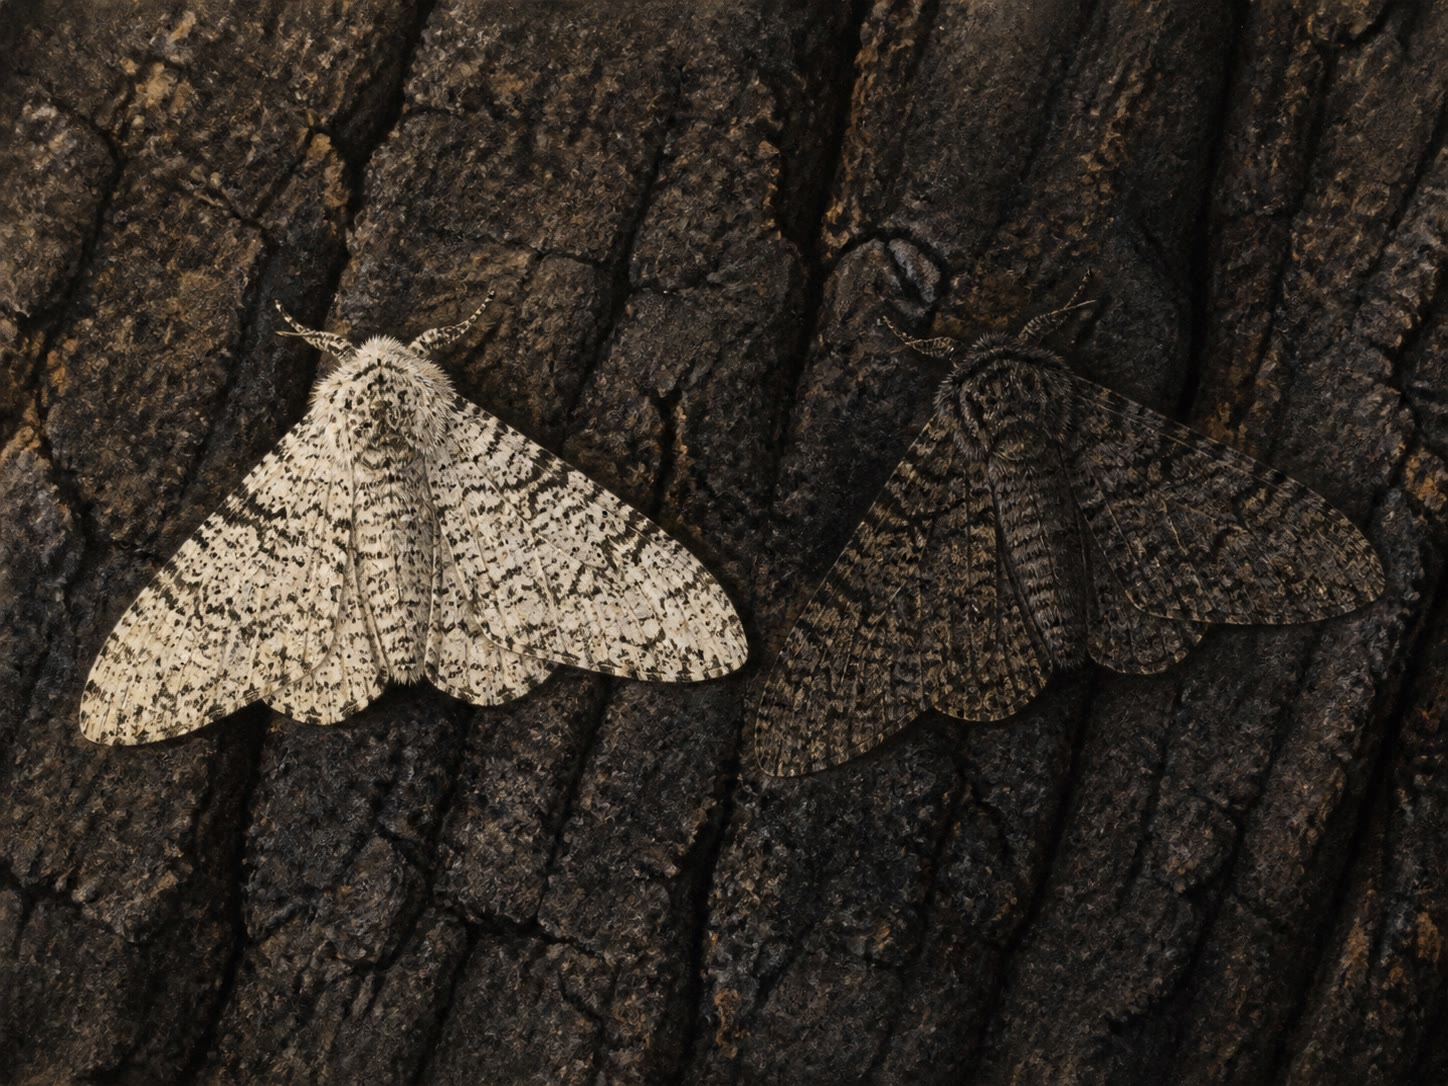
\includegraphics[width=0.56\linewidth]{images/book1/ai/g9-moths-bark.jpg}

{\small “检查”起作用时：在煤烟熏染的树皮上，浅色
型最为显眼——而最显眼的，
恰是被吃掉的那一只。}
\end{omfigure}

\begin{remark}[自然选择不是什么]\label{rem:g9:how-species-change:not}
三种长期存在的误解，予以摒弃：
\begin{itemize}
  \item \emph{无意图}：\omterm{def:g6:exploring-our-environment:conditions}{条件}的“选择”方式，
        正如潮\omterm{def:g6:exploring-our-environment:conditions}{湿度}“选择”鼠妇
        (\cref{ex:g6:exploring-our-environment:chooser})
        ——靠后果，而非抉择；没有任何东西在谋划；
  \item \emph{无完美}：选择只比较
        变异\emph{现存}者——它找到的是
        现有较优者，而非可想象的最优者（共同
        肢体蓝图的笨拙“改作他用”，
        \cref{exo:g9:evidence-of-evolution:7}，
        正是其标志）；
  \item \emph{努力不\omterm{def:g9:heredity-and-traits:heredity}{遗传}}：铁匠的
        手臂随铁匠一同死去；
        (\cref{prop:g9:heredity-and-traits:sorting});
        \omterm{prop:g9:how-species-change:selection}{自然选择}只作用于\omterm{def:g8:sexual-reproduction:gametes}{配子}所携带的内容。
        长颈鹿并非因把\omterm{def:g1:my-body:parts}{脖子}不断拉长——
        \omterm{def:g1:my-body:parts}{脖子}较长的变异个体取食更好、繁殖更多，
        胜过了较短者。
\end{itemize}
\end{remark}

\section{被观察与利用的引擎}

\begin{example}[医院中的选择]\label{ex:g9:how-species-change:resistance}
医学案例，按引擎的原理拆解，
供\cref{ch:g9:microbes-and-infection}使用：一个\omterm{def:g6:producing-our-food:fermentation}{微生物}
\omterm{def:g8:reproduction-and-environment:population}{种群}中存有少量具抗性的\omterm{prop:g9:genes-and-dna:explains}{突变}体
（\omterm{prop:g9:genes-and-dna:explains}{突变}零星产生）；抗生素充当“检查”；它
收走敏感个体，放过抗性个体，
这些个体便在病房中取而代之。以天计，而非以千年计——
世代以小时计，选择的速度与之成正比。
凡关于按疗程服完抗生素、不把抗生素
散布到农业中的规定，都是对引擎的管理：
检查时强时弱，你就会
培育出你本想要杀死的东西。
\end{example}

\begin{example}[人为干预“检查”的选择]\label{ex:g9:how-species-change:artificial}
\Cref{pb:g8:sexual-reproduction:1}中的育种者，
以她自己充当“检查”，运行同样的引擎——保留脆嫩
且抗病的，淘汰其余的。每一个犬种、每一种\omterm{def:g6:producing-our-food:farming}{作物}
品种、每一条奶牛品系，都是累积的
\emph{人工选择}：引擎力量的证明，
在人类的时间尺度上，从狼到玩赏犬，只需数千
代。达尔文——这位组装本章论证的博物学家——
在其巨著之首，
正是以这一比较起笔。
\end{example}

\begin{omfigure}
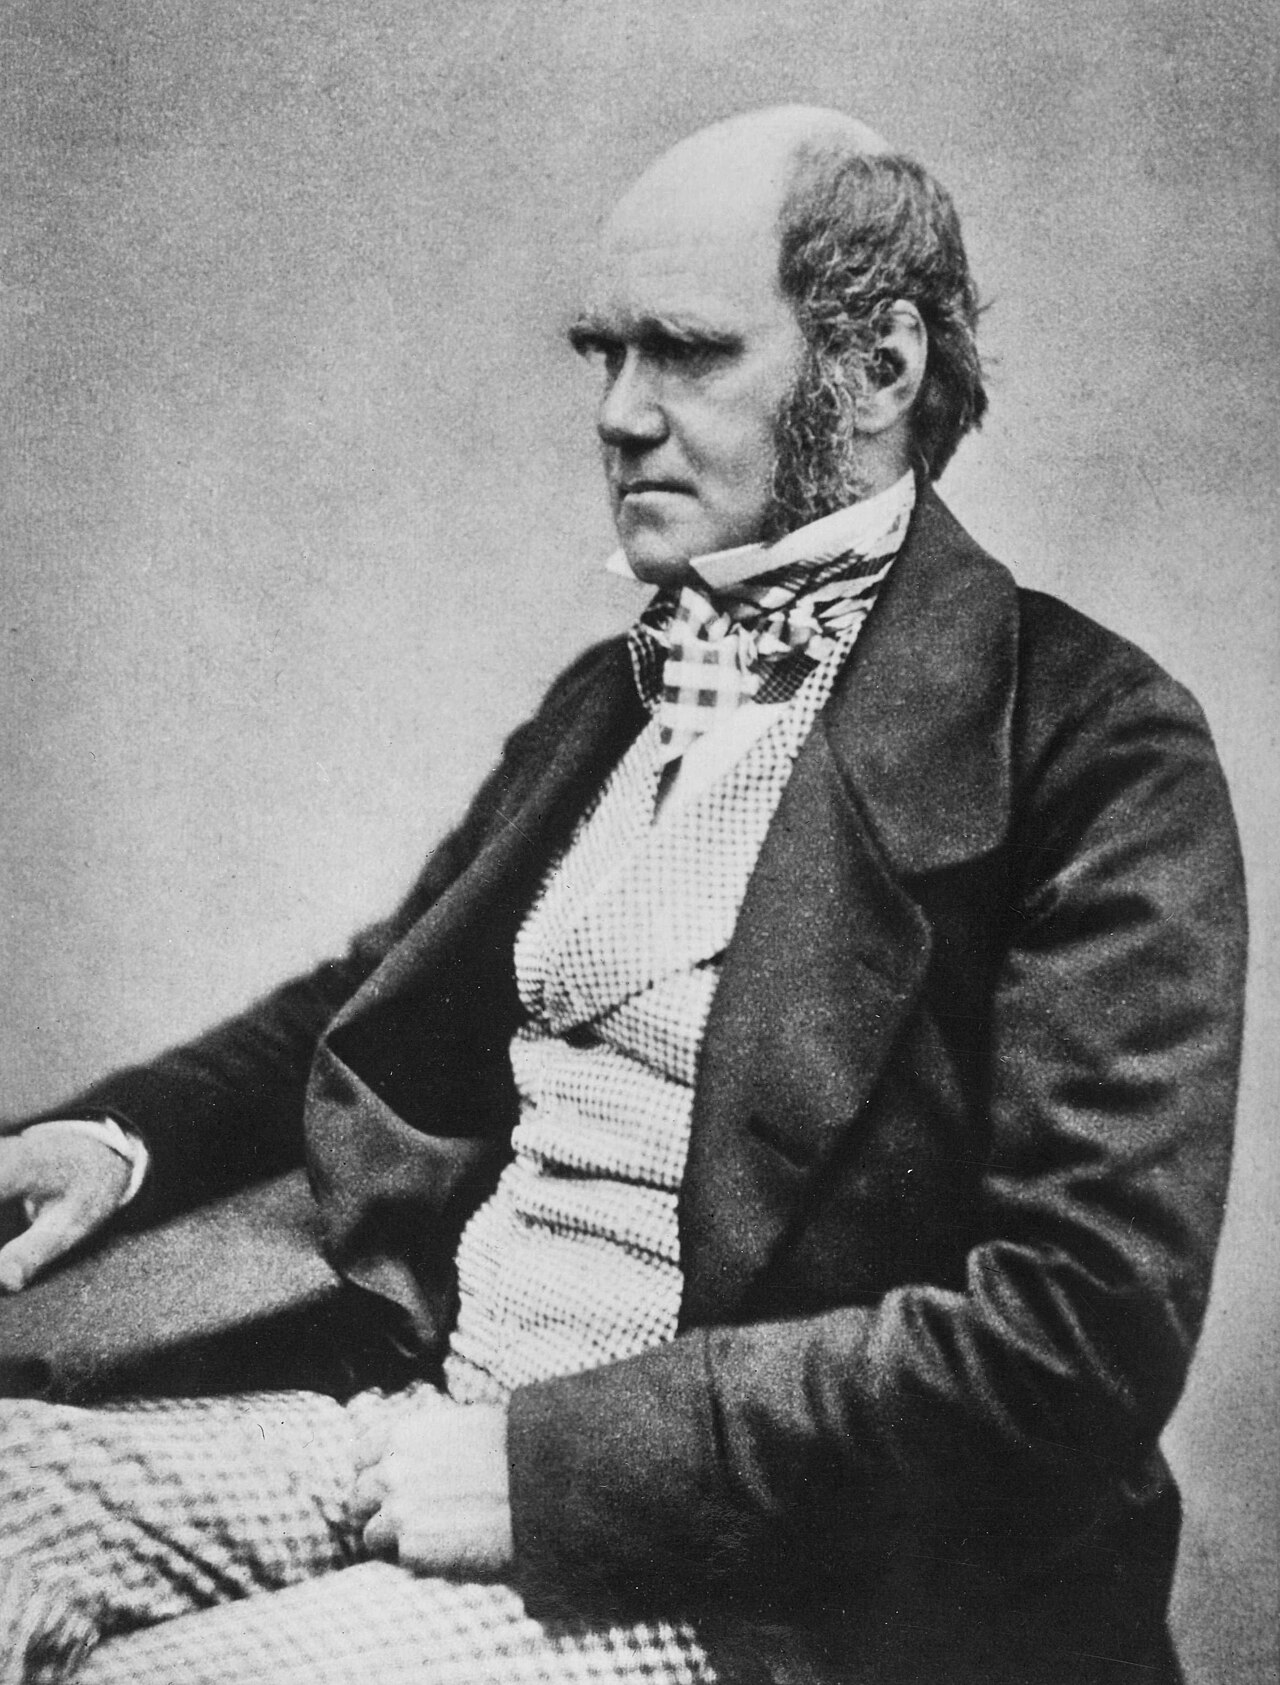
\includegraphics[width=0.42\linewidth]{images/book1/darwin.jpg}

{\small 查尔斯·达尔文，约摄于 1854 年，
正是他组织本章论证的那几年。}
\end{omfigure}

\begin{proposition}[从变化到新物种]\label{prop:g9:how-species-change:speciation}
\omterm{prop:g9:how-species-change:selection}{自然选择}解释了\omterm{def:g8:reproduction-and-environment:population}{种群}的变化；再加上一个要素，
便可解释\omterm{def:g8:reproduction-and-environment:population}{种群}的\emph{分裂}。
同一\omterm{def:g5:biodiversity:species}{物种}的两个\omterm{def:g8:reproduction-and-environment:population}{种群}被分隔开——海水上涨，
分布区一分为二，岛屿迎来漂流者
（\cref{exo:g6:how-plants-spread:11}）——两个\omterm{def:g8:reproduction-and-environment:population}{种群}各自运行
引擎，在各自的\omterm{def:g6:exploring-our-environment:conditions}{条件}下积累各自的
\omterm{def:g9:genes-and-dna:gene}{等位基因}。若分化足够充分，两者在相遇之处
不再相互杂交。依据
\cref{def:g5:biodiversity:species}的定义，两者
便成为原先一个\omterm{def:g5:biodiversity:species}{物种}所在之处的两个\omterm{def:g5:biodiversity:species}{物种}。系统树的分叉
（\cref{def:g6:classification-kinship:tree}）正是
这样的分裂，历经漫长岁月积累了无数次。
\end{proposition}
\admitted

\begin{method}[在任何案例中运行引擎]\label{met:g9:how-species-change:run}
对于任一声称的\omterm{prop:g9:how-species-change:selection}{演化}实例：
\begin{enumerate}
  \item 指出\emph{变异}，并检验其是否可\omterm{def:g9:heredity-and-traits:heredity}{遗传}
        （\cref{met:g9:heredity-and-traits:audit}）；
  \item 指出\emph{检查}，以及它如何
        在该变异中不均等地挑选个体；
  \item 追踪\emph{记账}：
        下一代中哪一方的\omterm{def:g9:genes-and-dna:gene}{等位基因}所占份额上升？
  \item 若为分裂，补充\emph{隔离}及
        分化的\omterm{def:g6:exploring-our-environment:conditions}{条件}；
  \item 检验时间尺度：世代而非年，才是
        引擎的“计时单位”。
\end{enumerate}
\end{method}

\section{练习}

\begin{exercise}[$\star$]\label{exo:g9:how-species-change:1}
陈述\omterm{prop:g9:how-species-change:selection}{自然选择}的三条事实及其
推论。
\end{exercise}

\begin{exercise}[$\star$]\label{exo:g9:how-species-change:2}
在蛾的案例中，指出变异、检查，以及
不均等的挑选——两个方向都要说明。
\end{exercise}

\begin{exercise}[$\star$]\label{exo:g9:how-species-change:3}
\omterm{prop:g9:how-species-change:selection}{自然选择}下发生变化的是个体，还是
\omterm{def:g8:reproduction-and-environment:population}{种群}？请说明理由。
\end{exercise}

\begin{exercise}[$\star$]\label{exo:g9:how-species-change:4}
请运用\omterm{prop:g9:how-species-change:selection}{演化}机制，纠正这一说法：“长颈鹿
伸长了\omterm{def:g1:my-body:parts}{脖子}，并把这种伸长\omterm{def:g9:heredity-and-traits:heredity}{遗传}下去。”
\end{exercise}

\begin{exercise}[$\star$]\label{exo:g9:how-species-change:5}
为什么抗生素抗性能在数天内\omterm{prop:g9:how-species-change:selection}{演化}，而蛾类
却要花费数十年？
\end{exercise}

\begin{exercise}[$\star$]\label{exo:g9:how-species-change:6}
苹果育种者与捕食蛾的\omterm{prop:g3:sorting-living-things:groups}{鸟类}有何共同之处，
又有何不同？
\end{exercise}

\begin{exercise}[$\star\star$]\label{exo:g9:how-species-change:7}
为什么\omterm{prop:g9:how-species-change:selection}{自然选择}无法产生“想象中最好的”
\omterm{def:g6:exploring-our-environment:components}{生物}体？其三条事实中哪一条构成了限制？
\end{exercise}

\begin{exercise}[$\star\star$]\label{exo:g9:how-species-change:8}
运用\cref{met:g9:how-species-change:run}分析雀鸟在
干旱中的情形（\cref{ex:g9:evidence-of-evolution:live}）：\omterm{def:g2:from-seed-to-plant:seed}{种子}
变硬，大喙能咬碎小喙咬不动的\omterm{def:g2:from-seed-to-plant:seed}{种子}。
\end{exercise}

\begin{exercise}[$\star\star$]\label{exo:g9:how-species-change:9}
梳理岛屿漂流者的\omterm{def:g5:biodiversity:species}{物种}形成过程，即
\cref{exo:g6:how-plants-spread:11}中的情形：
隔离、分化，以及可判定两者为两个\omterm{def:g5:biodiversity:species}{物种}的检验。
\end{exercise}

\begin{exercise}[$\star\star$]\label{exo:g9:how-species-change:10}
结合引擎的运作，解释为何未完成的抗生素
疗程与农场中随意散播的抗生素都会
催生抗性。
\end{exercise}

\begin{exercise}[$\star\star$]\label{exo:g9:how-species-change:11}
“\omterm{prop:g9:how-species-change:selection}{自然选择}，就是
\cref{ch:g8:reproduction-and-environment}中的检查，落在
\cref{ch:g9:unique-individuals}中的变异上。”
请论证这句话可以作为本书自身的总结。
\end{exercise}

\begin{exercise}[$\star\star\star$]\label{exo:g9:how-species-change:12}
为什么引擎\emph{需要}\omterm{def:g4:animal-reproduction:sexual}{有性生殖}的“洗牌”与\omterm{prop:g9:genes-and-dna:explains}{突变}的“涓流”——
在完全相同的克隆体\omterm{def:g8:reproduction-and-environment:population}{种群}中
（\cref{exo:g9:unique-individuals:8}），
一旦\omterm{def:g6:exploring-our-environment:conditions}{条件}改变，
\omterm{prop:g9:how-species-change:selection}{自然选择}会怎样？
\end{exercise}

\section{问题：岛屿笔记}

\begin{problem}[{周末问题——两个世纪的
火山群岛}]\label{pb:g9:how-species-change:1}
一个（综合历史素材改编的）群岛：
火山岛，从未与大陆相连，岛上栖息着形似雀类的鸟，
其喙的形状逐岛不同——
并且与其唯一明显的大陆近缘种不同。
博物学家的笔记跨越两个世纪。

\medskip\noindent\textbf{第一部分——规律。}
\begin{enumerate}
  \item 岛上只有能够跨海的\omterm{def:g5:biodiversity:species}{物种}：
        \omterm{prop:g3:sorting-living-things:groups}{鸟类}、漂流\omterm{def:g2:from-seed-to-plant:seed}{种子}、一种蝙蝠，没有
        本土陆生\omterm{prop:g3:sorting-living-things:groups}{哺乳动物}或青蛙。哪一章
        预测了这份“乘客名单”
        （\cref{exo:g6:how-plants-spread:11}）？
  \item 群岛上所有雀类都与那一种大陆\omterm{def:g5:biodiversity:species}{物种}相似，
        且相似程度超过地球上任何其他\omterm{prop:g3:sorting-living-things:groups}{鸟类}。
        \omterm{prop:g6:classification-kinship:kinship}{亲缘关系}推理
        （\cref{prop:g6:classification-kinship:kinship}）
        会对它们的起源得出什么结论？
  \item 喙形随岛上食物而异：\omterm{def:g2:from-seed-to-plant:seed}{种子}岛上为破壳的鸟，
        仙人掌岛上为探取的鸟。请读出
        这一对应关系，结合
        \cref{prop:g4:adapted-to-their-world:answers} ---
        再说明本章增加了\omterm{def:g4:adapted-to-their-world:adaptation}{适应}那一章所
        无法给出的内容。
  \item 为什么火山岛这类从未与大陆相连的岛屿
        恰是引擎的最佳展示场所？请指出它们
        大量提供的\omterm{def:g5:biodiversity:species}{物种}形成要素。
\end{enumerate}

\medskip\noindent\textbf{第二部分——
引擎的笔记年代。}
\begin{enumerate}[resume]
  \item 一个干旱年：软壳\omterm{def:g2:from-seed-to-plant:seed}{种子}歉收，硬壳\omterm{def:g2:from-seed-to-plant:seed}{种子}
        仍留存；捕鸟者的卡尺显示次年的
        雏鸟平均喙更深。请用引擎的
        核算方式推演这一描述。
  \item 随后是多雨年，软壳\omterm{def:g2:from-seed-to-plant:seed}{种子}回归，平均
        值随之回落。这一逆转
        对\omterm{prop:g9:how-species-change:selection}{自然选择}的“方向”说明了什么？
  \item 某岛的雀类被风暴带到另一座岛上，
        与当地居民的繁殖效果很差。
        这一现象正在检验哪一命题？
  \item 一本“神创论”时代的笔记提出异议：“从未有人
        见过一个\omterm{def:g5:biodiversity:species}{物种}变成另一个\omterm{def:g5:biodiversity:species}{物种}。”请结合
        时间尺度与多重证据汇合的方法
        作答（\cref{met:g9:evidence-of-evolution:weigh}）。
\end{enumerate}

\medskip\noindent\textbf{第三部分——综合
讲座。}
\begin{enumerate}[resume]
  \item 用引擎的
        五个步骤
        （\cref{met:g9:how-species-change:run}），讲述群岛从
        漂流者登岛到形成岛上\omterm{def:g5:biodiversity:species}{物种}的故事。
  \item 解释为何每座岛上的雀类都是“现有的较优者，
        而非可想象的最优者”——
        各岛的“牌库”能为\omterm{prop:g9:how-species-change:selection}{自然选择}提供什么？
  \item 将群岛与
        \cref{ex:g9:how-species-change:resistance}中的医院病房相联系：
        同一引擎，不同的运行速率——
        请说明决定速率的因素。
  \item 以达尔文的比较收束讲座，明确指出：
        养鸽人的手与干旱年的硬壳\omterm{def:g2:from-seed-to-plant:seed}{种子}
        有何共同之处。
\end{enumerate}
\end{problem}
